% !TEX root = ../main_lecture_notes.tex
\chapter{Introduction}\label{sec:introduction}

A blockchain is a distributed ledger maintained by achieving consensus among a number of nodes in a Peer-to-Peer network. The blockchain technology has attracted a lot of interest after the advent of the bitcoin cryptocurrency in 2008, see \citet{Na08}. Since then, the blockchain concept has been used to develop decentralized systems to store and maintain the integrity of time-stamped transaction data across peer-to-peer networks. Besides the creation of a digital currency, blockchain applications include the sharing of IT resources, the registration of authentication certificate or the implementation of smart contracts. \\

The topic of blockchain is of primary interest to computer scientists working on peer-to-peer networks and distributed algorithm. The problem of reaching consensus inside peer-to-peer networks is a classical problem framed as "The Byzantine general problem" by \citet{lamport1982the}. A group of generals from the Byzantine army is surrounding an enemy city. Communicating only by messenger, they must agree on a common battle plan. There may be traitors who will attack instead of retreat or non responding generals who will do nothing. For the project to be successful a majority of the general must either retreat or attack. The problem then reduces to finding an algorithm to ensure that the loyal generals reach an agreement. The problem is illustrated on \cref{fig:byzantine_general}.
\begin{figure}[!ht]
  \begin{center}
    \subfloat[Coordinated attack]{
      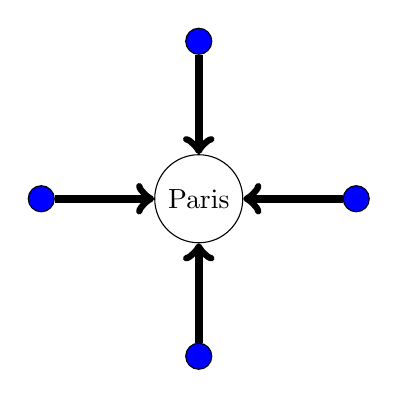
\begin{tikzpicture}[baseline]
\node[draw, circle] (P) at (0,0) {Paris};
\foreach \i in {(0,2), (0,-2), (2,0), (-2, 0)}{
		\node[draw, circle, fill = blue] (G) at \i {};
		\draw[->, line width=1mm,black] (G) -- (P);
	}
\end{tikzpicture}}
                         \hskip2em
    \subfloat[Failed attack due to one traitor and one non-responding general]{
      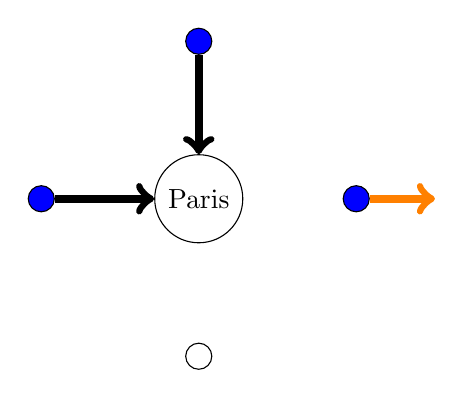
\begin{tikzpicture}[baseline]
\node[draw, circle] (P) at (0,0) {Paris};
\foreach \i in {(0,2),  (-2, 0)}{
		\node[draw, circle, fill = blue] (G) at \i {};
		\draw[->, line width=1mm,black] (G) -- (P);
	}

	\node[draw, circle, fill = blue] (G) at (2,0) {};
	\draw[->, line width=1mm,orange] (G) -- (3,0);
	\node[draw, circle] (G) at (0,-2) {};
\end{tikzpicture}}
    
    \caption{Illustration of the BYzantine general problem}
    \label{fig:byzantine_general}
  \end{center}
  \end{figure}

In a blockchain system, we have a large network of nodes that broadcast transactions which corresponds to pieces of information that will be written in the blockchain. light nodes, full nodes consensus and write information. 


\begin{itemize}
	\item Computer science
	\item Economics
	\item Applied math and operations research
\end{itemize}
\newpage